\section{Toolchain Analysis}
\label{sec:toolchain-analysis}

All the methods mentioned above start with a complete definition of the toolchain. In OpenETCS, the development of the toolchain follows an \emph{agile} approach.
Hence, for each (major) release we have to deal with an incomplete tool
chain. In addition to the methods of the previous section,  we need a qualification
process that can adapt to the development speed, deal with an incomplete toolchain
and can re-use qualification information.

Moreover, as stated by Asplund et al., the toolchain itself may
provide some mechanism that may reduce the tool qualification effort
\cite{asplund_towards_2012,asplund_qualifying_2012}. They are
descibred as a set of safety goals that the tool chain should ensure.
 In our context, most of the
tool integration effort is made by integrating tools into a tool
platform.  According to Asplund et al., the tool platform should
ensure the following safety-goals that will avoid some extra tool qualification:
\begin{itemize}
\item Coherent time stamp information: common time stamps on development artifacts.
\item Notification: the user should be notified when artifacts changed.
\item Data integrity:  avoid use of obsolete artifacts, the data used reflects the
  current state.
\item Data mining: all data used by safety analysis should be available and be
  verifiable.
\end{itemize}

\begin{figure}
\begin{center}
\begin{tikzpicture}[->, >=stealth,node distance=1.5cm, auto]
\tikzstyle{decision} = [diamond, draw, fill=blue!20, align=center]
\tikzstyle{block} = [rectangle, draw, fill=blue!20, align=center, rounded corners]
	\node [block] (n1) {Features Analysis};
	\node [block, below of=n1] (n2) {Toolchain Platform Analysis};
	\node [block, below of=n2] (n3) {Design Qualification Plan};
	\node [below of=n3] (sub3) {};
	\node [left of=sub3, node distance=4cm] (label1) {Toolchain \& Platform Development};
	\node [block, below of=label1, node distance=1cm] (n4) {Functional Specification};
	\node [block, below of=n4] (n5) {Code Development};
	\node [block, below of=n5] (n6) {Code Review};
	\node [block, below of=n6] (n7) {Testing};
	\node [block, right of=sub3, node distance=4cm] (n8) {Tools Evaluation};

	\node [below of=n8,align=center, node distance=2cm] (tq1) {Individual Tool Qualification\\(to be followed for each tool)};

	\node [block, below of=tq1, node distance=1.5cm] (tq2) {Operational\\Qualification};
	\node [block, left of=tq2, node distance=2.5cm] (tq3) {Installation\\Qualification};
	\node [block, right of=tq2, node distance=2.5cm] (tq4) {Performance\\Qualification};
	\begin{scope}[on background layer]
		\node [block, fit=(tq1) (tq2) (tq3) (tq4)] (n9) {};
		\node [block, fit=(label1) (n4) (n5) (n6) (n7)] (n10) {};
	\end{scope}
	\node [block, below of=n3, node distance=9cm] (n11) {Tool \& Platform Integration};
	\node [block, below of=n11] (n12) {Toolchain Installation Qualification};
	\node [block, below of=n12] (n13) {Toolchain Operational Qualification};
	\node [block, below of=n13] (n14) {Toolchain Performance Qualification};
	\node [block, below of=n14] (n15) {Maintenance};

	\draw[->] (n1) -- (n2);
	\draw[->] (n2) -- (n3);
	\draw[->] (n3) -- (n10);
	\draw[->] (n3) -- (n8);
	\draw[->] (n8) -- (n9);
	\draw[->] (n4) -- (n5);
	\draw[->] (n5) -- (n6);
	\draw[->] (n6) -- (n7);
	\draw[->] (n9) -- (n11);
	\draw[->] (n10) -- (n11);
	\draw[->] (n11) -- (n12);
	\draw[->] (n12) -- (n13);
	\draw[->] (n13) -- (n14);
	\draw[->] (n14) -- (n15);
\end{tikzpicture}
\end{center}
\caption{Qualification process as proposed by Izaskun de la Torre}
\label{fig:qualification_process_idelatorre}
\end{figure}

\begin{figure}
\begin{center}
\scalebox{0.9}{
\begin{tikzpicture}[->, >=stealth,node distance=1.5cm, auto]
\tikzstyle{decision} = [diamond, draw, fill=blue!20, align=center, font=\footnotesize]
\tikzstyle{block} = [rectangle, draw, fill=blue!20, align=center, rounded corners]
	\node [block] (n1) {Features Analysis};
	\node [block, below of=n1] (n2) {Toolchain Platform Analysis};
	\node [below of=n2,align=center] (l1) {Individual Tool Qualification (to be followed for each tool)};
	\node [block, below of=l1, node distance=1cm] (n3) {Define Process \& Usage Context};
	\node [block, below of=n3] (n4) {Tool Classification};
	\node [decision, below of=n4, anchor=north] (d1) {Tool is\\prequalified};
	\node [below of=d1, node distance = 3cm] (subd1) {};
	\node [block, left of=subd1, node distance=4.5cm] (n5) {Check conformance\\with defined process\\and usage context};
	\node [decision, right of=subd1, node distance=4.5cm] (d2) {Qualification\\by third party\\possible};
	\node [block, below of=d2, node distance=3cm] (n6) {Provide process and usage context\\for third party qualification};
	\node [decision, below of=d1, node distance= 3cm] (d4) {Conformance?};
	\node [decision, below of=d4, node distance=3cm] (d3) {Tool is\\open source};
	\node [below of=d3, node distance = 2.53cm] (subd3) {};
	\node [block, fill=red!20, right of=subd3, node distance=2.5cm] (n7) {Qualification impossible\\(except ``proven in use'')};
	\node [block, left of=subd3, node distance=2.5cm] (n8) {Operational Qualification\\by Tool Chain Integrator};
	\node [block, below of=d4, node distance=8cm] (n9) {Tool-to-Platform Integration Qualification};
	\begin{scope}[on background layer]
		\node [block, fill=black!10, fit=(l1) (n3) (n4) (d1) (n5) (d2) (n6) (n9)] (individual_quali) {};
	\end{scope}
	\node [block, below of=n9] (n10) {Toolchain Installation Qualification};
	\node [block, below of=n10] (n11) {Toolchain Operational Qualification};
	\node [block, below of=n11] (n12) {Toolchain Performance Qualification};

	\draw[->] (n1) -- (n2);
	\draw[->] (n2) -- (individual_quali);
	\draw[->] (n3) -- (n4);
	\draw[->] (n4) -- (d1);
	\draw[->] (d1) -- node [near start] {yes} (n5);
	\draw[->] (d1) -- node [near start] {no} (d2);
	\draw[->] (d2) -- node [near start] {yes} (n6);
	\draw[->] (d2) -- node [near start] {no} (d3);
	\draw[->] (d3) -- node [near start] {no} (n7);
	\draw[->] (d3) -- node [near start] {yes} (n8);
	\draw[->] (n5) -- (d4);
	\draw[->] (d4) -- node [near start] {no} (d2);
	\draw[->] (n8) -- (n9);
	\draw[->, out=190, in=180] (d4) to node [near start] {yes} (n9);
	\draw[->, out=-50, in=0] (n6) to (n9);
	\draw[->] (individual_quali) -- (n10);
	\draw[->] (n10) -- (n11);
	\draw[->] (n11) -- (n12);
\end{tikzpicture}}
\end{center}
\caption{Proposed adaptation by Stefan Rieger (among other changes, the TC development branch was removed as this work is not part of qualification itself)}
\label{fig:qualification_process_idelatorre}
\end{figure}

\section{Scenario-based Qualification of Individual Tools}
\label{sec:scenario-based-tool-quali}

Qualifying a toolchain always requires the qualification of the individual tools it is comprised of. The effort required depends on the type and license of the tool to be qualified. To this end in the following we have identified a number of different scenarios that are of relevance in the context of the openETCS project as depicted in Figure~\ref{fig:tool-qualification-scenarios}.

\begin{figure}
\begin{center}
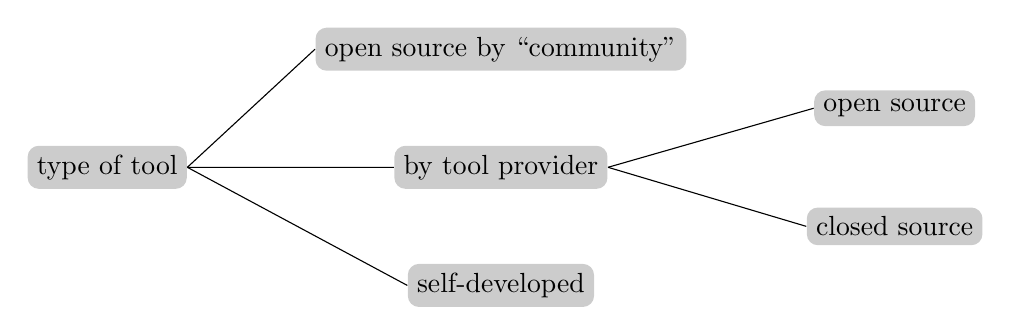
\begin{tikzpicture}[parent anchor=east,child anchor=west,grow=east, edge from parent, level distance=5cm]
	\tikzstyle{every node}=[fill=black!20,rounded corners]
	\node {type of tool}
		child { node {self-developed} }		
		child { node {by tool provider}
			child { node {closed source} }
			child { node {open source} }
		}
		child { node {open source by ``community''} };
\end{tikzpicture}
\end{center}
\caption{Scenarios to consider when qualifying individual tools}
\label{fig:tool-qualification-scenarios}
\end{figure}

In the following considerations for the individual scenarios are described.

\subsection{Self-developed Tool}

For a self-developed tool the project needs to provide the means for qualification and quality assurance. As the tool has not been employed in productive use by others the ``proven in use'' argument \textcolor{red}{[Remark: It needs to be checked whether this argument actually applies to EN 50128]} does not apply.

\subsection{Tool Provided by a Tool Provider}

For tools provided by a third party we must distinguish again two cases:

\paragraph{The tool is provided as closed source tool}

If the tool is not pre-qualified by the tool provider the options are limited. If the tool provider is not willing or unable to provide the means for qualification, the qualification of the tool will be almost impossible. One exception might be if the tool is already in use on a broad scale in industry and is generally regarded as reliable for the intended purpose. Also the tool class must be considered here.

\paragraph{The tool is provided as open source}

In this case it would be possible to adapt the tool and analyse it to enable qualification. However, this involves a huge amount of effort which is best done by the tool provider who as a better insight into the tool's internal workings. Also a third party who has already experience with the tool or is a specialist with regards to qualifying safety-critical tools could be entrusted with the qualification task.

\subsection{Open Source Tool Provided by the ``Community''}

If no tool provider can be identified but the tool is developed by the community and distributed under an open source license, the tool qualification has to be conducted by the project. However, many open source tools have a large development and expert community which can certainly be of help. In addition, the ``proven in use'' argument could possibly be applied (e.g., for tools like GCC).


\section{OpenETCS Toolchain Qualification Process}
\label{sec:toolchain-qualification-process}

The OpenETCS tool chain  will be defined by the set of its features and
a guideline describing how to correctly use it.
A SysML block diagram describes the tool chain architecture at a certain point in time as shown in
Figure \ref{fig:overview}. 
\begin{figure}[htbp]
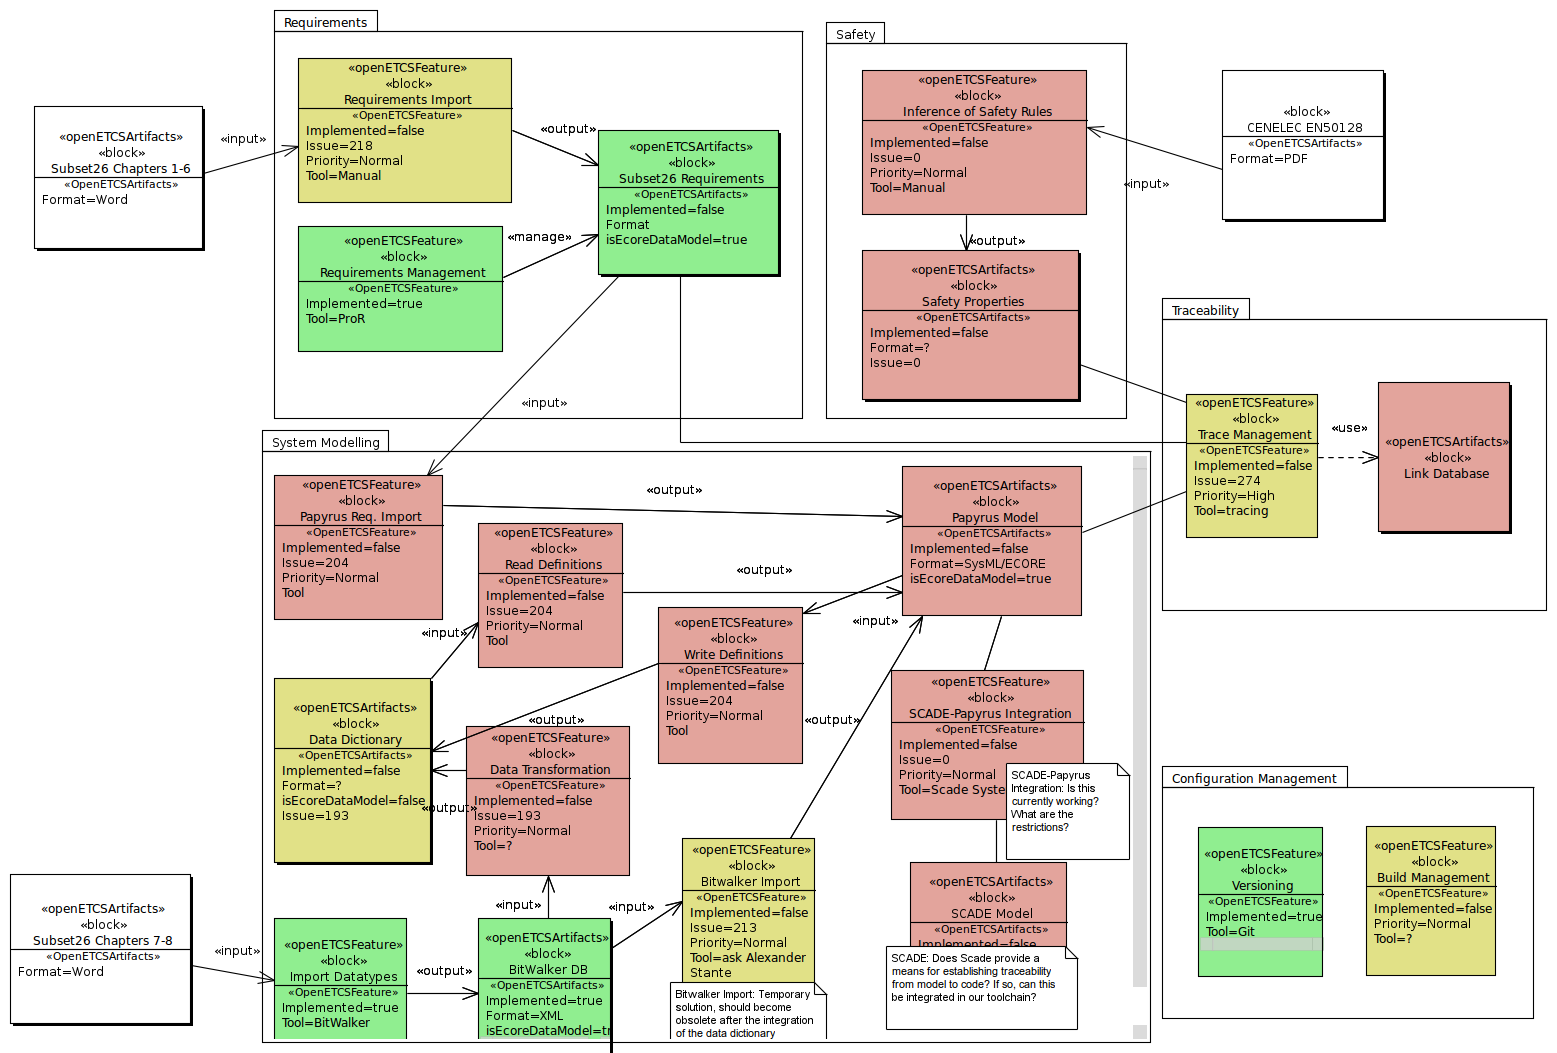
\includegraphics[width=\textwidth]{ToolChainmodel}
\caption{\label{fig:overview} Tool Chain overview (20.02.14) -- \\
  Green Block: Implemented \\
  Yellow Block: Work in Progress \\
  Red Block: Not started \\
  White Block: External Artifacts} 
\end{figure}

This block diagram is intended to grow according to new feature requests and the
needs of openETCS participants.  This diagram will be kept updated
as a reference of our tool chain. In any case, the complete information
regarding the feature availabilities  may be found in the Eclipse product
definition.

Each feature of the toolchain is a block with the profile ``openETCSFeature''
and  each artifact is block with the profile ``openETCSArtifact''.  Each
feature realizes at least one use case and may be implemented by one or more tools.
Note that in the tool platform features  may also be
implemented as plug-ins. The diagram also imposes a (partial) order
on the tasks. While some may be done in parallel, many tasks are dependent on others.
Currently, the diagram neither highlights the use of the tools, nor the order of actions
to be performed. This diagram should be completed by guidelines on
how to use the tool chain and/or an activity diagram.

To mitigate the qualification process, we will first consider more
than one feature at a time considering that errors from a tool A may
be detected by a Tool B in the next step of the tool chain process.
Furthermore, the toolchain is a collection
of features and not only tools. This differs from Asplund and al. in the sense that
some of the tool integration mechanisms that automate transformation of data, represent features
 and are thus not out of the scope of the qualification.

Due to our development process, a ``pre-qualification'' of tools should be made
when integrating a tool.

\todo[inline]{This high-level list should be detailed.}
\paragraph{Tool Integration Process for Qualification}

\begin{itemize}
\item Define name and version
\item Describe use cases
\item Provide justification of the tool within the tool chain
\item Provide input/output artifacts format (associated with the
  version)
\item Integrate the tool in the SysML model
\item Provide tool manual and other available documentation (associated with the version)
\item Link with an issue tracker
\end{itemize}

One possible implementation is to represent all these in formations
directly in the SysML model.

\todo[inline]{This high-level list should be detailed.  What I would expect: Which artefacts exist; How they are connected; When artefacts have to be re-validated (e.g. due to changes); What roles exist; who is responsible for what; etc.}
\paragraph{The Qualification Process}

\begin{enumerate}
\item Feature Analysis
  \begin{itemize}
  \item This step should assign a class to each feature based on the use cases.
  \item Define the potential errors
  \item Identify counter measure and/or error detection
  \item For T3 tools 2 alternatives:  certified compiler/generator or
    object code checker and/or exhaustive tester
  \end{itemize}
\item Tool platform  analysis 
  \begin{itemize}
  \item Provide evidence that the safety-goals mentioned in the
    previous sub-section are fulfilled\textcolor{red}{[The identification of safety goals is missing in step 1]}
  \end{itemize}
\item Toolchain Analysis
  \begin{itemize}
  \item Defines the work-flow
  \item Identify the ``hot spots'' of the toolchain
  \item Rearrange the toolchain if possible
  \item Find new measures when needed with combining tools (redundancy with orthogonal
    codes \ldots{})
  \end{itemize}
\item Toolchain qualification verification 
  \begin{itemize}
  \item Check consistency of tool version with  manuals and other
    provided feature information
  \item Generate table to  check if all possible errors has a
    detection or a correction mechanism
\item Generate the qualification report
  \end{itemize}

\end{enumerate}







